\chapter{Bidirectional Long Short Term Memory Network Models}
In this chapter, we first describe the fully structured BiLSTM model: the state-of-the-art model combining BiLSTM with Character Embeddings and Conditional Random Fields (CRF). Then, we show the performance and decoding speed of BiLSTM models with different configurations on POS and NER.

\section{Model Description}
\subsection{Bidirectional Bidirectional Long Short Term Memory}

Recurrent neural networks (RNNs) (\citeauthor{mikolov2010recurrent}, \citeyear{mikolov2010recurrent}) have shown impressive results on sequence tagging tasks. RNNs can keep the future and the past data persistent by using memory cells with loops in them. However, RNNs are biased towards the most recent data in practice. Long Short Term Memory Networks (LSTMs), special RNNs with Long Short Term memory cells  (\citeauthor{graves2005framewise}, \citeyear{graves2005framewise}), are designed to combat the bias problem. LSTMs learn long dependencies in a sequence with the help of Gates (\citeauthor{graves2005framewise}, \citeyear{graves2005framewise}). Gates control how much of the input information to pass to the next LSTM cell, and how much of the previous information to forget.

Given a sentence with $n$ words each of which is represented as a dense vector $x_i$, a LSTM makes use of $x_{1:n}$ to compute a forward representation $\overrightarrow {h_{i}}$ for the $i$th word. In general, computing a backward representation $\overleftarrow {h_{i}}$ would be useful for sequence tagging. Bidirectional LSTM (BiLSTM) is an extension to LSTM which takes into account both the past elements and the future elements in a sequence. A BiLSTM generates both $\overrightarrow {h_{i}}$ and $\overleftarrow {h_{i}}$ for the $i$th word in a sequence. The hidden embedding $h_{i}$ is the concatenation of $\overrightarrow {h_{i}}$ and $\overleftarrow {h_{i}}$. BiLSTM mapping is defined as $BiLSTM_{\theta}$:
$h_{i} = BiLSTM_{\theta}\left(x_{1:n}, i\right)$ where $\theta$ represents trainable parameters in BiLSTM. Figure \ref{fig:bilstm} illustrates the application of the BiLSTM model on an NER example.

\begin{figure}
  \centering
  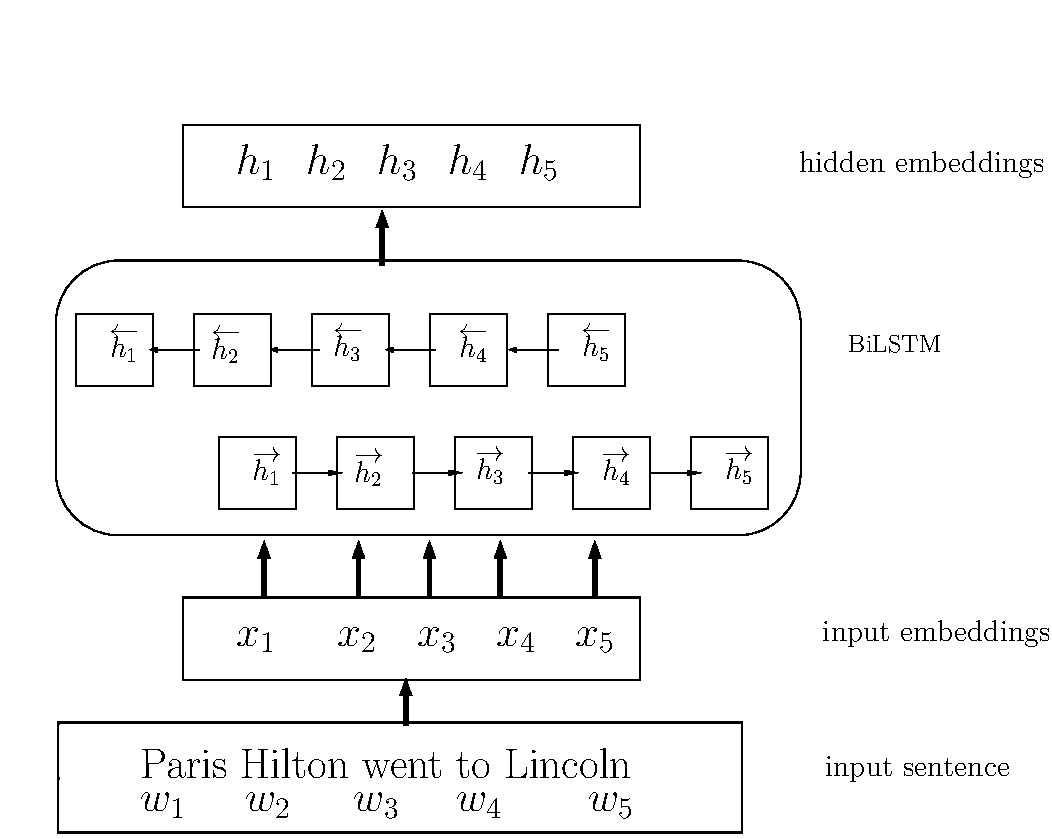
\includegraphics[scale=0.6]{bilstm.pdf}
 \caption{The architecture of BiLSTM on an NER example}
  \label{fig:bilstm}
\end{figure}

\subsection{Character Embeddings}

Instead of using hand-engineered features listed in Chapter 2 (like prefixes and the suffixes of a word), we can use a BiLSTM network to construct word representations from characters in it (\citeauthor{lample2016neural}, \citeyear{lample2016neural}). This architecture is denoted as Character Embeddings. It has been shown that learning character embeddings has been found useful for capturing morphological evidence (\citeauthor{ling2015finding}, \citeyear{ling2015finding}). Figure \ref{fig:charlstm} describes the architecture using character embeddings and BiLSTM to generate word embedding for word ``Paris''. The input to the BiLSTM is the letter sequence of a word. We define a character dictionary which maps each character to a $d$-dimensional vector representation. The English character dictionary contains uppercase and lowercase letters, numbers, and punctuation. We look up each $c_{i}$ of the input letter sequence from the dictionary and get the character embedding vectors $X:\left\{x_{1},x_{2},\dots,x_{n}\right\}$. Then, character embedding vectors $X$ are fed into BiLSTM to generate forward and backward hidden embeddings of the character sequence. We concatenate the last forward hidden embedding $\overrightarrow {h_{n}}$ and the last backward hidden embedding $\overleftarrow {h_{1}}$ with the embeddings from word embedding dictionary lookup to obtain the final word embedding.

We add Character Embeddings in the sequence tagging system by concatenating the output of Character Embeddings and the word embeddings from lookup to form input embeddings. Then, we feed the input embeddings to BiLSTM and CRF, and we get the fully structured BiLSTM model (BiLSTM-CRF) for sequence tagging. The character embeddings and word embeddings are learned together during training. There are existing implementations of BiLSTM-CRF, such as NeuroNet by \cite{2017neuroner} which achieves state-of-the-art performance. In order to compare BiLSTM-CRF with other models in this thesis, we re-implement the model.

\begin{figure}
  \centering
  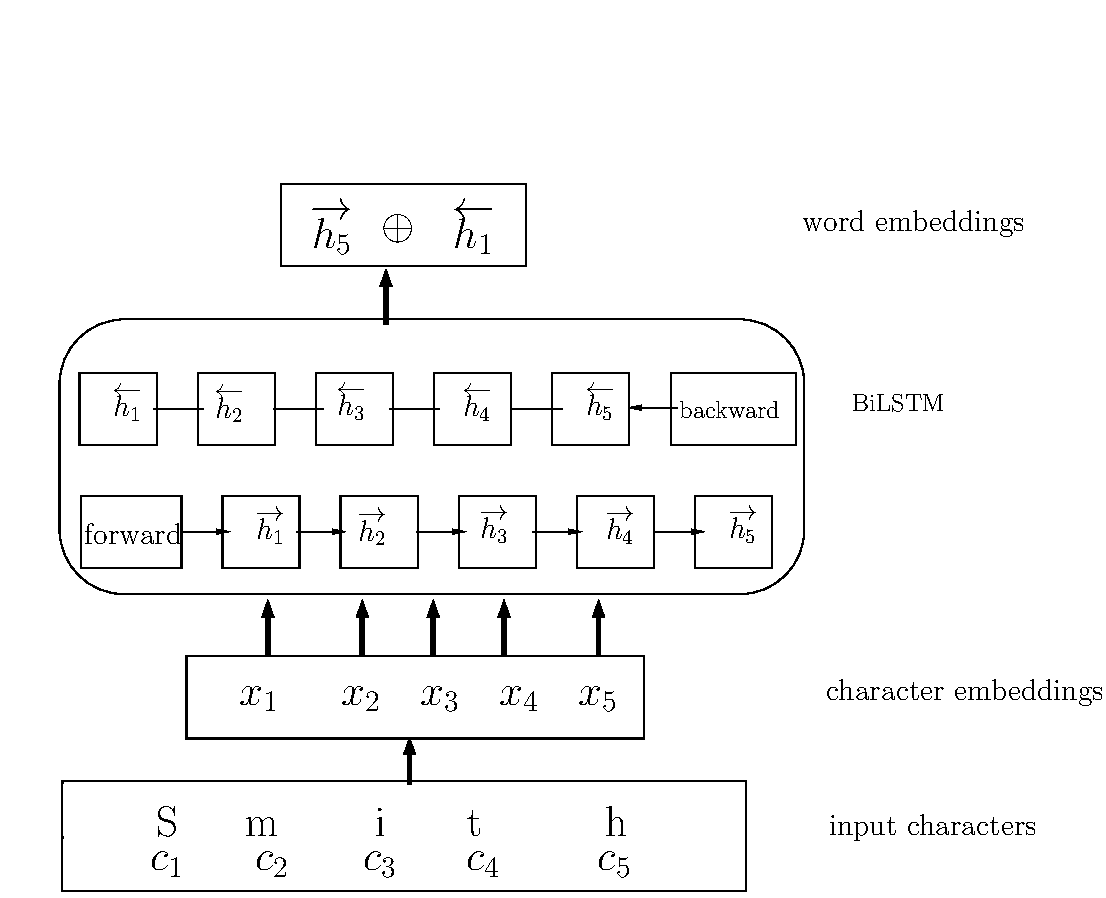
\includegraphics[scale=0.6]{bilstmchar.pdf}
 \caption{The word embedding derived from the character embeddings}
  \label{fig:charlstm}
\end{figure}

\subsection{Conditional Random Fields}

Conditional Random Fields (CRF) models make decisions on sentence levels instead of making independent decisions on each word. We combine the BiLSTM model with a CRF layer to form the BiLSTM-CRF model. The architecture of BiLSTM-CRF is shown in Figure \ref{fig:bilstmcrf}. 

\begin{figure}[h]
  \centering
  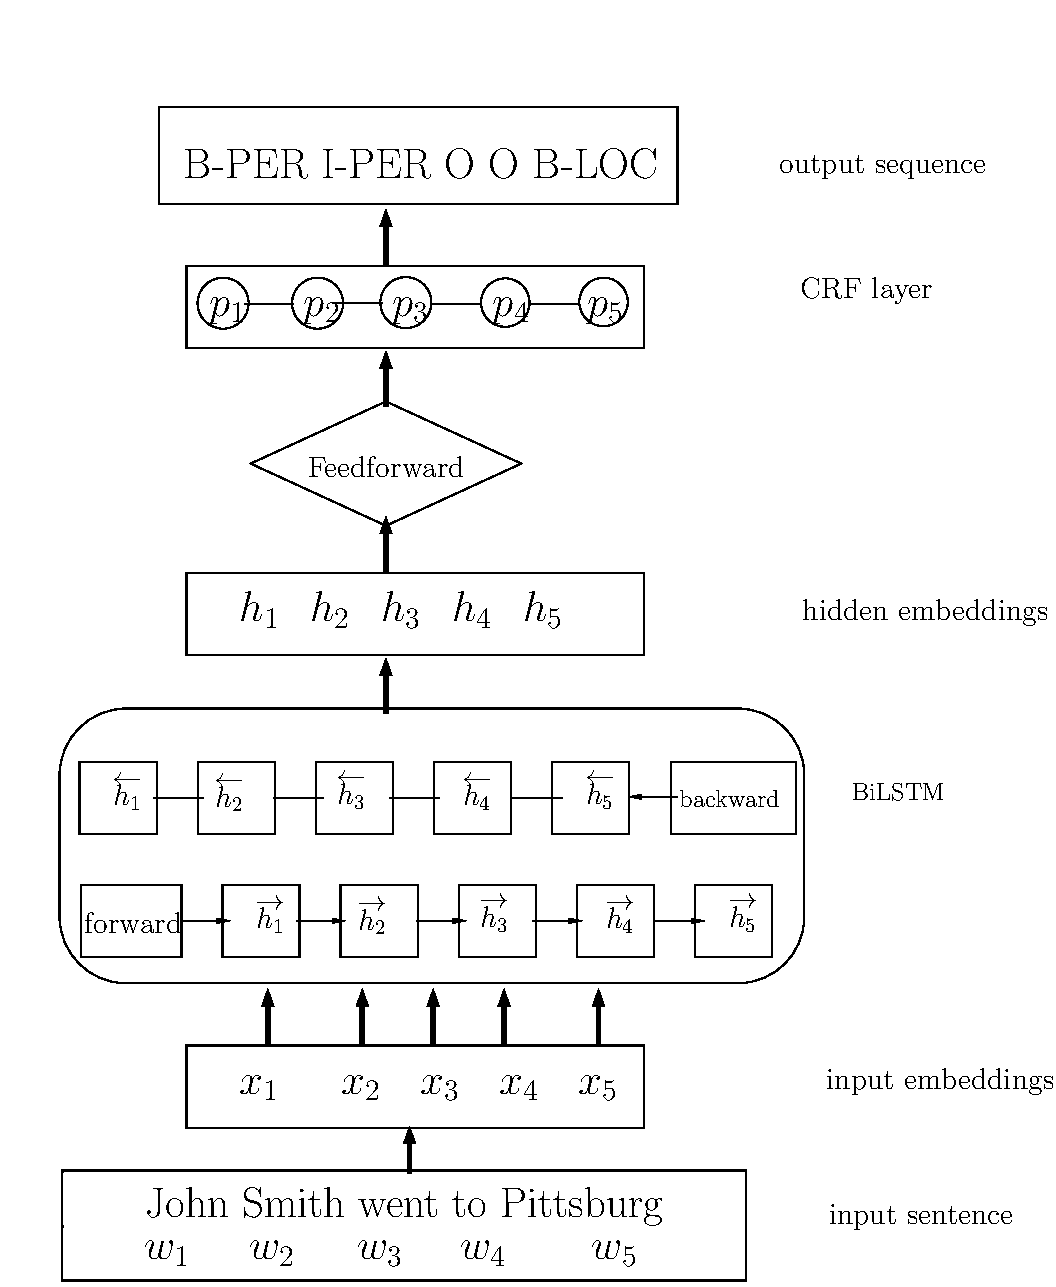
\includegraphics[scale=0.6]{bilstmcrf}
 \caption{The architecture of BiLSTM-CRF on an NER example}
  \label{fig:bilstmcrf}
\end{figure}

In BiLSTM-CRF, given a sequence of output predictions $y=\left( y_{1},y_{2},\ldots y_{n}\right)$, the score of the output sequence is:

\begin{equation}
S\left( y\right)=\sum _{i}^{n}T_{i,i+1}+\sum _{i}^{n}p_{i}\left(y_{i}\right)
\end{equation}

\noindent
where $T$ is a matrix of transition scores such that $T_{i,j}$ represents the score of a transition from the label $i$ to label $j$, and $p_{i}\left(y_{i}\right)$ is the probability of $y_{i}$ being the label of word $i$.

During training, we score every possible output sequence, and use a softmax layer (\citeauthor{dugas2001incorporating}, \citeyear{dugas2001incorporating}) to generate the probability distribution of output sequences: $P\left( y\right) = \textit{softmax}(S\left( y\right))$. Then, we minimize the negative log likelihood over the training sentences. During decoding, we can recover the tag sequences of test data using dynamic programming. Thereby, decoding time grows quadratically in the number of tag types, and grows linearly in the number of sentences.

\section{Experiments and Results}

To evaluate BiLSTM models, we run BiLSTM with three configurations on POS, NER, and Chunking: BiLSTM with word features only (BiLSTM); BiLSTM with Character Embeddings (BiLSTM-Char); BiLSTM with Character Embeddings and a CRF layer (BiLSTM-CRF). We report the performance and decoding speed of the models on Penn Treebank data set for POS, CoNLL 2003 data set for NER, CoNLL 2000 data set for Chunking. The details of the data sets are shown in Table \ref{table:my-dataset}.

\begin{table}[h]
\centering
\caption{Experiments Specification}
\label{table:hardware}
\begin{tabular}{|c|c|}
\hline
CPU & Intel i7-5820k \\ \hline
GPU & NIVID GeForce GTK 1080 \\ \hline
OS & Ubuntu 16.04.03 \\ \hline
CUDA & 8.0 \\ \hline
Tensorflow & 1.0 \\ \hline
Python & 2.7.13 \\ \hline
\end{tabular}
\end{table}

\begin{table}[h]
\centering
\caption{Hyperparameters used in BiLSTM Models}
\label{table:hyperparameters2}
\begin{tabular}{|c|c|}
\hline
Hyperparameters & Values \\ \hline
character embedding size & 50 \\ \hline
word embedding size & 100 \\ \hline
feedforward layer size & 200 \\ \hline
feedforward layer & 1 \\ \hline
BiLSTM layer size & 100 \\ \hline
BiLSTM layer & 2 \\ \hline 
optimizer & Adam \\ \hline
learning rate & 0.01 \\ \hline
batch size & 32 \\ \hline
dropout & 0.5 \\ \hline
\end{tabular}
\end{table}

The experiments were conducted on a Linux server with a single 10G Nvidia GeForce GPU. The experiment specifications are shown in Table \ref{table:hardware}. We use the hyperparameters defined in NeuroNER  (\citeauthor{2017neuroner}, \citeyear{2017neuroner}), which uses BiLSTM-CRF for NER and is shown to achieve near the state-of-the-art performance. Since dropout training (\citeauthor{hinton2012improving}, \citeyear{hinton2012improving}) can improve the performance by encouraging the model to depend on both character embeddings and word embeddings, we apply a dropout mask on the input embeddings before the BiLSTM layer. The dropout rate is set to 0.5 in the experiments. Table \ref{table:hyperparameters2} shows the hyperparameters used in BiLSTM models. We use the pretrained word embeddings from GloVe which contains 40K words, and initialize all the weight parameters using Xavier initialization (\citeauthor{glorot2011domain}, \citeyear{glorot2011domain}).

\begin{table}[h]
\centering
\caption{Performance of BiLSTM Models on POS}
\label{table:lstm-table1}
\begin{tabular}{|c|c|c|}
\hline
Model         & Accuracy  & Error Reduction (words)      \\ \hline
BiLSTM  & 96.1     & $-$                            \\ \hline
BiLSTM-Char & 97.21 (+1.11) & 629             \\ \hline
BiLSTM-CRF & \textbf{97.34} (+1.24)  & 702             \\ \hline
\end{tabular}
\bigskip
\caption{Performance of BiLSTM Models on NER CoNLL 2003 Data}
\label{table:lstm-table2}
\begin{tabular}{|c|c|c|c|}
\hline
Model  & Precision & Recall & F1      \\ \hline
BiLSTM  & 84.27 & 83.22 & 83.74     \\ \hline
BiLSTM-Char & 87.07 & 88.81 & 87.93 (+4.19)\\ \hline
BiLSTM-CRF & 89.93 & 90.16 & \textbf{90.05} (+6.31)  \\ \hline
\end{tabular}
\bigskip
\caption{Performance of BiLSTM Models on Chunking}
\label{table:lstm-table3}
\begin{tabular}{|c|c|c|c|}
\hline
Model  & Precision & Recall & F1      \\ \hline
BiLSTM  & 91.26 & 92.33 & 91.79    \\ \hline
BiLSTM-Char & 92.51 & 93.45 & 92.98 (+1.19)\\ \hline
BiLSTM-CRF & 93.91 & 93.81 & \textbf{93.86} (+2.07)  \\ \hline
\end{tabular}
\end{table}


\begin{table}[h]
\centering
\caption{BiLSTM Models Decoding Speed (words/sec)}
\label{table:lstm-table4}
\begin{tabular}{|c|c|c|c|}
\hline
Model       & POS & NER (CoNLL 2003) & Chunking    \\ \hline
BiLSTM-CRF    & 9009     & 10100   &5390\\ \hline
BiLSTM-Char        & 13992 (1.55$\times$)    & 11271 ($\times$1.12) &6616 ($\times$1.23) \\ \hline
BiLSTM             & 23036 (2.56$\times$)   & 20740 ($\times$2.05)  &10321 ($\times$1.91)\\ \hline
\end{tabular}
\end{table}

Table \ref{table:lstm-table1}, Table \ref{table:lstm-table2} and Table \ref{table:lstm-table3} describe the final performance of BiLSTM models on the POS, NER and Chunking. Table \ref{table:lstm-table4} reports the decoding speed of BiLSTM models. In terms of performance, the fully structured BiLSTM model outperforms the other two. Compared to BiLSTM, the structure of Character Embeddings increases the performance, but BiLSTM networks do not heavily depend on features other than words. CRF layer is more helpful for NER than POS and Chunking. In terms of decoding speed, it is obvious that the more features the model has, the slower it would be. Adding a CRF layer will increase the performance but decrease the decoding speed. 

